Two sets of features are extracted from the motion picture image to be used in the classifier:

\begin{enumerate}
\item Hu Moments;
\item Changes in the area of the extracted object over time.
\end{enumerate}

\subsubsection*{Hu Moments}

Hu set of invariant moments is used as the first set of features. In order to calculate Hu moments, motion history image for a given video clip is first built\footnote{this is done by using modified version of sample code from OpenCV. Original code is available at \url{https://code.ros.org/trac/opencv/browser/trunk/opencv/samples/python/motempl.py}}. Motion history image is built from black and white images reconstructed from contour images. This is done by combining them into one image by superimposing them. Example motion history images for "rock", "paper" and "scissors" signs are shown in Figure \ref{fig:mhir}, Figure \ref{fig:mhip} and \ref{fig:mhis} respectively. 

Hu moments are then extracted from motion history image and used as features of the motion image.

\begin{figure}
\begin{center}
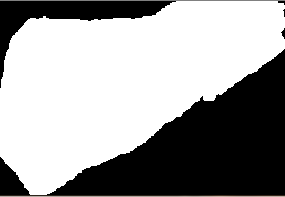
\includegraphics[width=80mm]{mhi_rock.png}
\caption{Motion history image for "rock" sign.}
\label{fig:mhir}
\end{center}
\end{figure}

\begin{figure}
\begin{center}
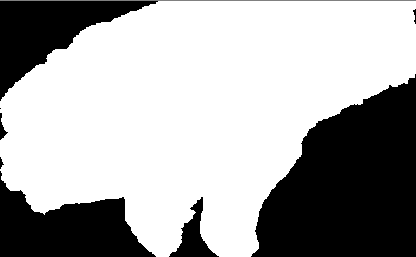
\includegraphics[width=80mm]{mhi_paper.png}
\caption{Motion history image for "paper" sign.}
\label{fig:mhip}
\end{center}
\end{figure}

\begin{figure}
\begin{center}
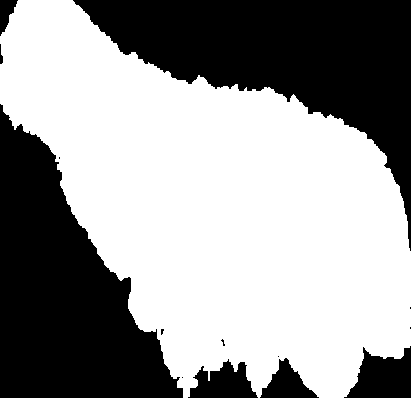
\includegraphics[width=80mm]{mhi_scissors.png}
\caption{Motion history image for "scissors" sign.}
\label{fig:mhis}
\end{center}
\end{figure}

\subsubsection*{Temporal function of the object size}

In addition to Hu moments, additional set of five features is generated by temporarily dividing provided video clip into five equal segments and calculating average area taken by the hand in each of these segments. This way we can see how area of the hand in the image changes over time and represent such changes as features usable by the classifier. 

While being a simple method, it explains large amount of variance between different signs. 